\documentclass[11pt]{article}[twocolumn]
\usepackage{fullpage}
\usepackage{hyperref}
\hypersetup{breaklinks=true}
\urlstyle{same}  % don't use monospace font for urls
\usepackage{graphicx}
\usepackage{float}
\usepackage{calc}
\usepackage{ifthen}
\usepackage{tikz}
\usepackage{booktabs}
\usepackage{multirow}
\usepackage{siunitx}

\providecommand{\tightlist}{%
	\setlength{\itemsep}{0pt}\setlength{\parskip}{0pt}%
}

\begin{document}

\title{\textbf{Detecting Bannable Content on Reddit}} \\
\author{Kelly Gothard, David Matthews, Nicholas Hanoian, Colin Sandberg}
\maketitle

\hrule
\section{Introduction}
Socially destructive and unhealthy communities can thrive on social networks, particularly on Reddit.  Reddit is a platform that hosts pages, or subreddits, that are defined by a topic/interest area where users can post and reply to other posts, creating threads.  These topic areas are created by users, for users, and topics such as fat-shaming, white supremacy, sexual violence, etc, have taken root into Reddit.  Reddit's response to these communities is to restrict their activity, whether that be through temporary or permanent bans.

Our goal is to create a model for Reddit's banning patterns for the purpose of automatic detection of ``bannable'' content.  We explore various algorithms, units of text, and transformations to determine the best model for detecting bannable subreddits.

\section{Data}
The data, all Reddit comments posted in October of 2016, was acquired from pushshift.io\footnote{\url{https://files.pushshift.io}}. This dataset is maintained by Jason Baumgartner and has been used in many areas of research (Gaffney, 2018). In this dataset, each line is represented a comment, and each comment had an author, the subreddit it was posted to, the body of the text, the timestamp that it was posted, and other comment attributes.  We labeled the data by referencing a list of banned subreddits, and labeling comments in our dataset that were posted onto those banned subreddits as `banned', and all others as `not banned'.  

\subsection{Representations of Data}
We test various units of text from subreddits to explore the best ways to describe the content that is contained in a subreddit.  We defined the following units of text as potentially useful ways to represent content in a subreddit:
\begin{itemize}
    \item Comment; a single comment is posted by a single author, and has one body of text.  Many comments exist within a subreddit.
    \item Thread; a thread is made up of a tree of comments that are replies to other comments.  Subreddits can contain many threads, and threads can contain many comments.
    \item 200 words; to standardize amount of training information per training example, we construct a 200 word model wherein comments are stitched together and trimmed so that each training example contains 200 words. For more details see Section \ref{sect:200WordModel}.
    \item Subreddit; we can take all of the comments in a subreddit and treat them as one large corpus to describe the subreddit.
\end{itemize}


The distribution of words per unit of text is crucial, because the features in each of our models are the words in the corpora.  Each of the distributions shown in Figure \ref{fig:words_per_unit_of_data} below have a right-skewed distribution of words, where most comments, threads, and subreddits have far fewer words than those that have the most.  The distribution for 200 words is not shown below, because each unit of text contains 200 words and is therefore a uniform distribution.

\begin{figure}[H]
    \caption{Distributions of Words per Unit of Text: Comments, Threads, and Subreddits}
    \centering
    \begin{subfigure}{\textwidth}
        \centering
        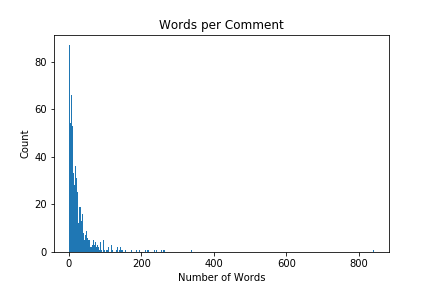
\includegraphics[width=0.31\textwidth]{comment_word_dist.png}
    \end{subfigure}
    \begin{subfigure}{\textwidth}
        \centering
        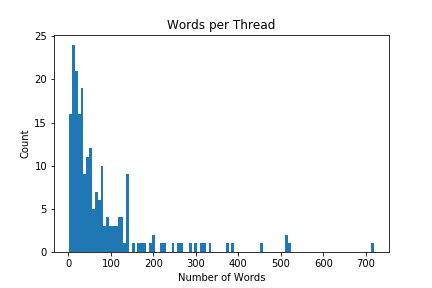
\includegraphics[width=0.31\textwidth]{thread_word_dist.png}
    \end{subfigure} 
    \begin{subfigure}{\textwidth}
        \centering
        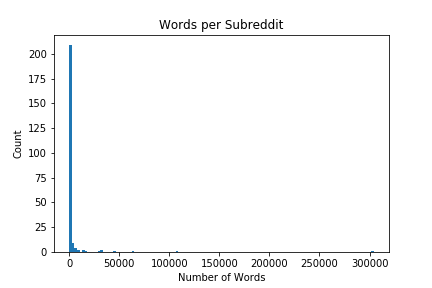
\includegraphics[width=0.31\textwidth]{subreddit_word_dist.png}
    \end{subfigure} \\
    \label{fig:words_per_unit_of_data}
\end{figure}

\subsection{200-Word Representation}
\label{sect:200WordModel}

In addition to the heavily right-skewed distribution in the word count length of each comment, thread, and subreddit, these units of data also include many training examples which are ambiguous. For example, the text ``too bad he wasn't'' forms a complete comment in a banned subreddit. Despite this comment appearing in a banned subreddit, the comment by itself is not harmful and could easily appear in a not banned subreddit. It would be unreasonable to assume that a model could accurately classify comments like this one as originating from a banned or not banned subreddit.

To counteract this issue we propose a new data representation consisting of 200-word chunks of continuous text built from comments. For example, if we are given a stream of comments from a subreddit, we can form the 200-word representation by doing the following. Read words from comments until we build up a buffer of 200 words. This becomes the first example. Then we continue to read words from where we left off, building up another buffer of 200 words. This becomes the second example. This process repeats until we have split all of the words within a given subreddit into 200-word chunks.

This length of data was chosen to help mitigate the problems of short text ambiguity. Although longer data would further reduce this ambiguity, it would also further reduce the already small number of banned training examples. Two hundred words was chosen to balance these two competing objectives.

From the first 10 million comments in the month of October, 2016 we formed two groups: a train group consisting of a random 80\% of the comments and a test group consisting of the remaining 20\% of the comments.
For the training group, we divide the comments into two subgroups of banned and not banned comments and construct the 200-word unit training examples from each of these subgroups.
For the testing group we divide the comments by subreddit and construct the 200-word unit test examples from each of these subgroups.


\subsection{Feature Engineering}

By using the words as features in our models, we assume that the occurrence of each word has a some weighted relationship with the bannable-ness of a unit of text.  We know that some words that are associated with illegal and/or socially destructive are mostly unique to those contexts, and will likely occur far less often in subreddits that should likely not be banned.  We can give these words extra weight as features by computing their rank divergence, or difference in rank, between two corpora.  We compute rank divergence by ranking each words in two corpora by their frequency, where the most frequent words have the lowest rank | words like `the' might have rank of 1 | and words that are less frequent have higher rank.  If we subtract the rank of a word in one corpus from the rank of that same word in another corpus, we have a normalized measure of the difference in frequency of a word between two corpora.

For example, Figure \ref{fig:rankshift} below shows the log of rank by the log of rank divergence.  Words in corpora of banned and not banned subreddits were ranked by frequency, and rank divergence was calculated. Each point on the plot is a word, and the points that are labelled along the bottom edge are words that had the lowest rank (or highest frequency) at each value of rank divergence.  The word ``fat'' has a notably low rank compared to other words at that value of rank divergence (~1000).  This is an indicator that this word might be unique to the bannable subreddit corpus, and thus might be useful identifier.

\begin{figure}[H]
    \caption{Log of Rank Divergence by Log of Rank and Top 15 Words with Highest Rank Divergence}
    \centering
    \begin{subfigure}{\textwidth}
        \centering
        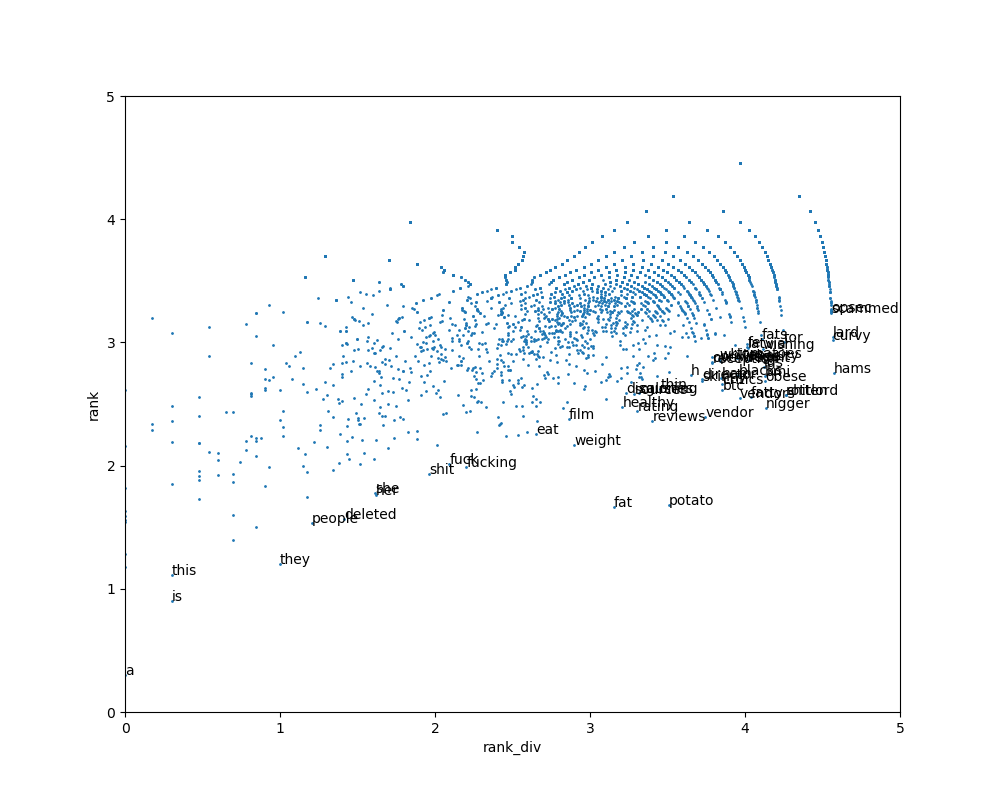
\includegraphics[width=0.6\textwidth]{rankdiv_scatter.png}
    \end{subfigure}
    \begin{subfigure}{\textwidth}
        \centering
        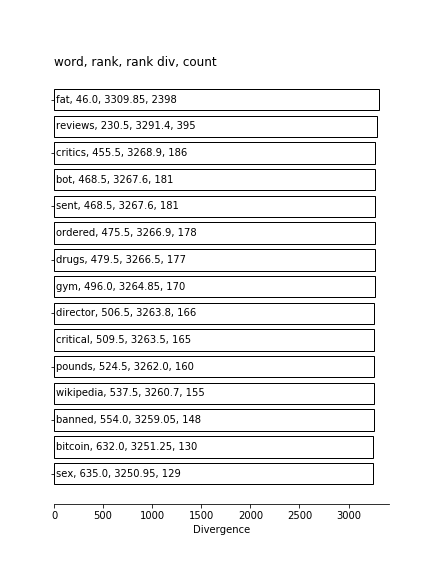
\includegraphics[width=0.37\textwidth]{Subreddits_rankdiv_shift.png}
    \end{subfigure}  \\
    \label{fig:rankshift}
\end{figure}

Figure \ref{fig:rankshift} also shows the words in our dataset, sorted by rank divergence and filtered by rank.  These words appear to be potentially related to bannable activity on Reddit, such as illegal sales (`bitcoin', `drugs') as well as spam (`bot', `reviews') and fat shaming (`fat',`pounds').  We propose applying a matrix transformation of rank divergence for each word to its TF-IDF representation as a method of augmenting data to improve detection of bannable subreddits.

\section{Results}

\subsection{Support Vector Machine, Naive Bayes, and Rank Divergence Models}

We used each representation of text data, sampling not banned data to create a balanced set, for training and testing of a support vector machine and a na\"ive Bayes classifier.  Note that each representation used to train the models were also the representations of the testing set | models trained on comments predicted only on comments, models trained on threads predicted only on threads, and so on.  This moves away from our overall goal of classifying subreddits, but we wanted to start off as simple and rudimentary as possible before adding complexity to our method of classification.  We address this issue later on when using neural networks.


We found that comments, subreddits, and threads did not perform well with these models while 200 words per subreddit did perform well.  We included results for comments, threads, and subreddits in appendices below, and move forward with only the 200 words per subreddit representation.  The 200 word chunks likely performed better than the other corpus types because, due to the uniform distribution of words per training unit, we ultimately gain more information than by looking at posts, threads, or subreddits alone.  This is because a majority of comments, threads, posts have very few words, so by taking the first 200 words from a subreddit, we overcome encountering sparse threads or comments as representations of a subreddit.

Figure 4 below shows the F1 score for the bannable class from cross validation of a na\"ive Bayes model without the rank divergence transformation, na\"ive Bayes with the transformation, SVM without transformation, and SVM with transformation.

\begin{figure}[H]
    \caption{Na\"ive Bayes vs SVM, with and without Rank Divergence}
    \centering
    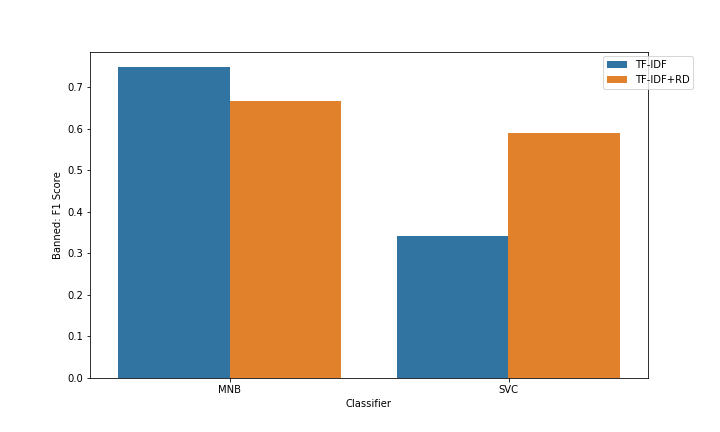
\includegraphics[width=0.5\textwidth]{words200_clf_barplot.png}
\end{figure}

The highest performing model was the na\"ive bayes that did not use the rank divergence transformation.  This model had an F1 score of 0.80 for the not-banned class and 0.75 for the banned class, as shown in Figure 5.  The na\"ive bayes model with no rank divergence transformation, trained on 200 word chunks performed the best out of the other corpus types, algorithms, and transformed models.

We also find that the rank divergence does not improve the na\"ive bayes model, but does improve the SVM.  However, the SVM still does not perform as well as na\"ive bayes without the transformation.

\begin{figure}[H]
\begin{center}
\caption{Naive Bayes: Testing 10-fold Cross Validation Classification Report}
\begin{tabular}{|l|r|r|r|r|r}
\hline
    & Precision & Recall & F1-Score & Support \\
    \hline
    Not-Banned  & 0.72 & 0.90 & 0.80 & 1000\\
    Banned  & 0.86 & 0.66 & 0.75 & 1000\\
    \hline
    Accuracy  &  &  & 0.78 & 2000\\
    Macro Avg  & 0.79 & 0.78 & 0.77 & 2000\\
    Weighted Avg  & 0.79 & 0.91 & 0.77 & 2000\\
    \hline
\end{tabular}
\end{center}
\end{figure}

\begin{figure}[H]
\begin{center}
\caption{Naive Bayes: Testing 10-fold Cross Validation Confusion Matrix}
\begin{tabular}{|r|r|r|r|}
    \hline
    & & \multicolumn{2}{c|}{Actual}\\
        \hline
    \multirow{3}{*}{Predicted} &
    & Not-Banned & Banned \\
    \hline
    & Not-Banned  & 896 & 104\\
    & Banned  & 341 & 659\\
    \hline
\end{tabular}
\end{center}
\end{figure}

The results in Figures 4 and 5 were promising, but we felt that we could improve our detection of bannable subreddits by using more data and by using neural networks for classification.  Additionally, the models above predict bannability of 200 word chunks, not subreddits as a whole.  In the next section, we modify the way we construct our testing data such that we train on 200 word chunks but predict on subreddits.

\subsection{Neural Network-based Model}

\begin{figure}
    \centering
    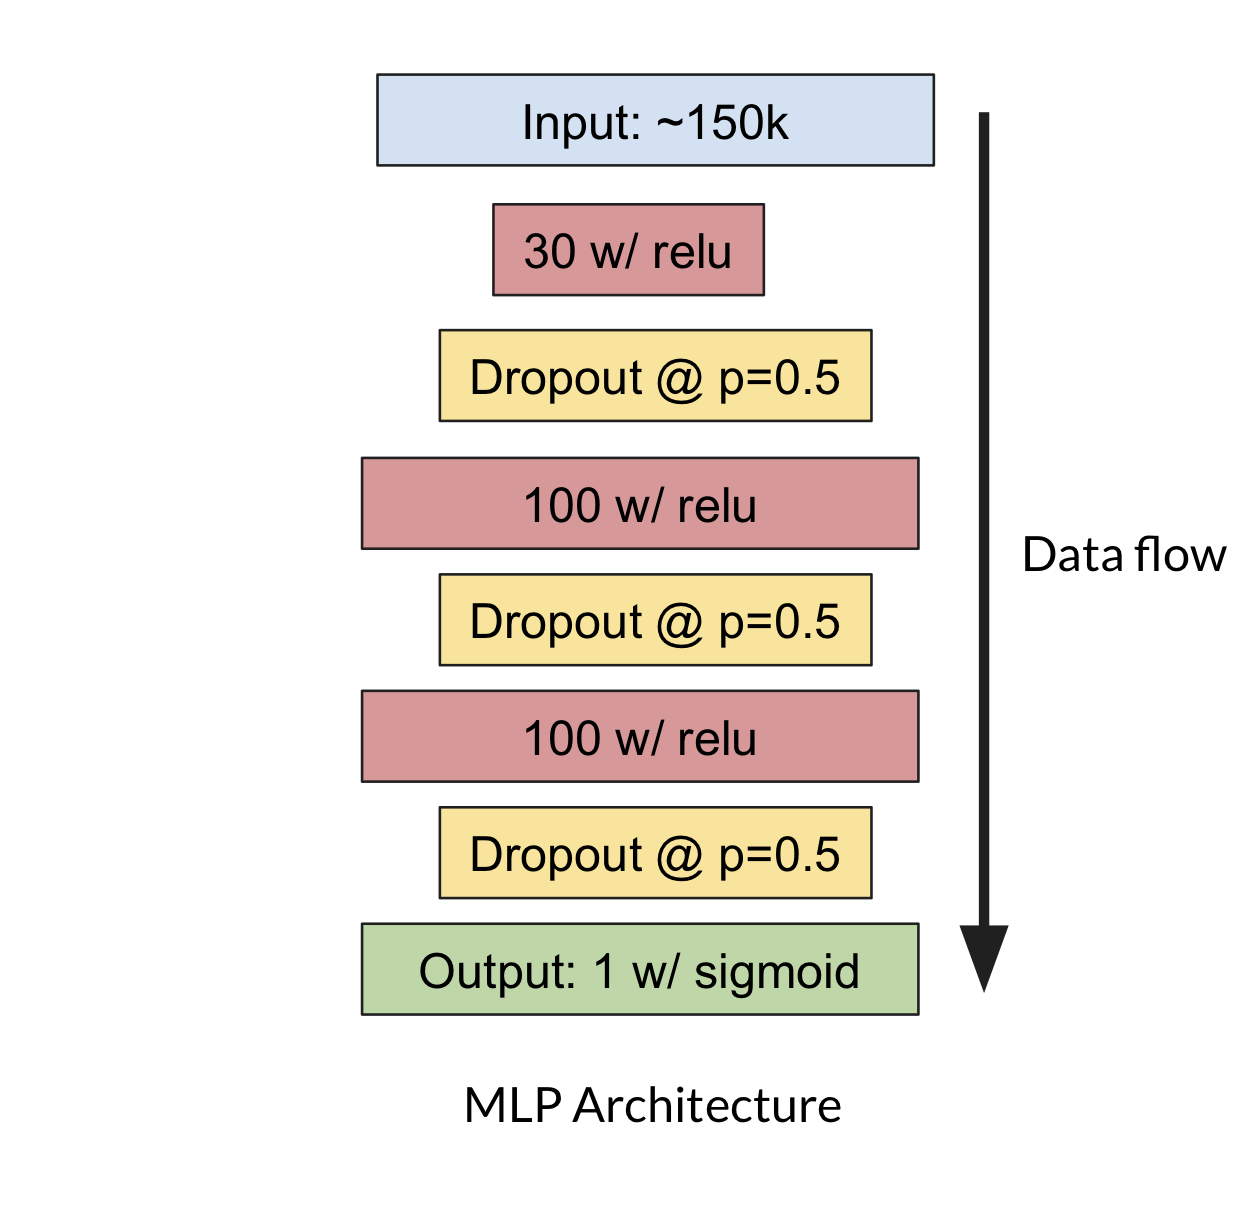
\includegraphics[width=0.55\linewidth]{MLP_Architecture.png}
    \caption{Architecture of the Multi-Layer Perception used herein.}
    \label{fig:MLP_Architecture}
\end{figure}

Using the 200-word unit, we aim to create a model which does a better job of classifying subreddits as bannable or not. The non-neural models all do a fairly poor job of classifying individual 200-word chunks, even on balanced data. Hence, we first sought out increased performance by using a more complex model in the form of a neural network. The model architecture is fairly simple, and is as described in Figure \ref{fig:MLP_Architecture}. It is a multiplayer perceptron with 3 hidden layers, ReLu activation between each, and an output layer of 1 neuron with a sigmoid activation. In between each fully-connected layer and the next we add a dropout layer with $p=0.5$ in order to prevent overfitting. We initially trained this network on balanced data and found that it performed much better than the non-neural methods. However, we still do not classify 200 word units well when using unbalanced data.

The initial model used the binary cross-entropy loss function which is the standard to use for a binary classifier. The unbalanced class problem led us to research other loss functions that do a better job of learning on unbalanced data. We settled on using focal loss which is designed to handle the training of neural networks on data that is extremely unbalanced, just like ours. It does a better job on this data by placing a much higher emphasis on the samples from the class that are not well-classified. 

This focal loss-based model performs excellently on balanced training and validation data, achieving F1 scores greater than 0.8. This appears to be excellent, especially when compared to simpler models, but in fact it is not very useful because when evaluated on fully unbalanced data, its performance plummets. However, since we are using the focal loss function, we can train effectively on unbalanced data. In order to be able to compare models with difference class imbalance ratios, we always validate on balanced data.

We first tried to use training data representative of the true data, but we found that this model was unable to achieve any significant results with validation data. This is likely due to the limitations of our model architecture. We then tried other class imbalance ratios to see how high we could get, while still maintaining appropriate performance. We found that a good ratio for our model to learn on was 20 not banned examples for every banned example. This achieved a training F1 score of 0.936, and a validation F1 score (on balanced data) of 0.524 after training for approximately 15 epochs. This performance may seem poor, but this is the performance for just one example. 

For our actual goal of classifying subreddits, each subreddit has multiple chunks of 200 words that we can look at. In order to classify each subreddit, we run each 200-word chunk through the model, obtaining an output between 0 and 1. All of a subreddit's outputs are then averaged together giving us an aggregate measure of whether the subreddit should be classified as banned or not banned. The only step remaining is to decide on the threshold that decides between banned and not banned.


In order to allow us to choose a threshold without biasing our results, we create a separate split of our data which we refer to as the threshold dataset. We then compute the aggregate measure for each subreddit in this threshold dataset, as described above. To pick a threshold, we consult the ROC curve, as shown in Figure \ref{roc}. In our case, we want to maximize the true positive rate while not decreasing the false positive rate too much. This is because we want recall to be high so that we can pass an over-sampled list of possible bannable subredits to moderators for further review. For this reason, we considered thresholds ranging from 0.001 to 0.25. After considering the tradeoff between increasing recall and decreasing precision, we settled on a threshold of 0.01, as it offered good performance on the threshold dataset. The performance of this cutoff on the threshold dataset is shown in Figures \ref{threshold-classification} and \ref{threshold-confusion}.

Finally, to see the actual performance of our model, we run it on a new, unseen testing set of subreddits and their associated 200-word chunks. We take the average of the outputs from each subreddit and compare it to our threshold value of 0.01. We look at the performance of the full model on the testing set in Figures \ref{test-classification} and \ref{test-confusion}. The model performed extremely well on this test set, successfully recalling 12 out of 15 banned subreddits, and achieving an overall macro average recall of 0.86.


\begin{figure}[H]
    \caption{Focal Loss Model: ROC Curve}\label{roc}
    \centering
    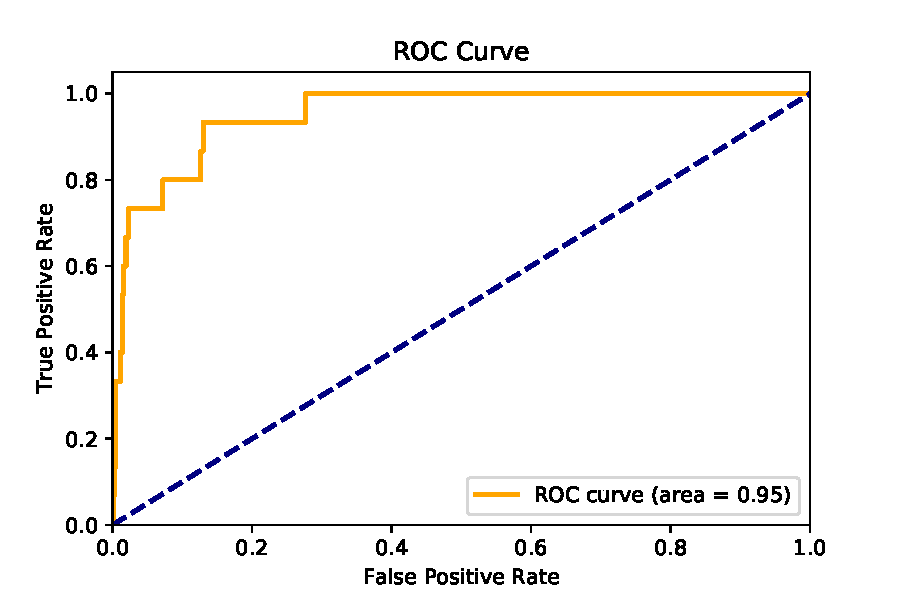
\includegraphics[width=0.6\textwidth]{roc(2).pdf}

\end{figure}

\begin{figure}[H]
\begin{center}
\caption{Focal Loss Model: Threshold Dataset Classification Report}\label{threshold-classification}
\begin{tabular}{|l|r|r|r|r|r}
\hline
    & Precision & Recall & F1-Score & Support  \\
    \hline
    Not-Banned  & 1.00 & 0.91 & 0.95 & 2692\\
    Banned  & 0.05 & 0.87 & 0.09 & 269\\
    \hline
    Macro Avg  & 0.52 & 0.89 & 0.66 & 2961\\
    \hline
\end{tabular}
\end{center}
\end{figure}


\begin{figure}[H]
\begin{center}
\caption{Focal Loss Model: Threshold Dataset Confusion Matrix}\label{threshold-confusion}
\begin{tabular}{|r|r|r|r|}
    \hline
    & & \multicolumn{2}{c|}{Actual}\\
        \hline
    \multirow{3}{*}{Predicted} &
    & Not-Banned & Banned \\
    \hline
    & Not-Banned  & 2690 & 2\\
    & Banned  & 256 & 13\\
    \hline
\end{tabular}
\end{center}
\end{figure}
 
\begin{figure}[H]
\begin{center}
\caption{Focal Loss Model: Testing Classification Report}\label{test-classification}
\begin{tabular}{|l|r|r|r|r|r}
\hline
    & Precision & Recall & F1-Score & Support \\
    \hline
    Not-Banned  & 1.00 & 0.92 & 0.96 & 2700\\
    Banned  & 0.05 & 0.80 & 0.09 & 262\\
    \hline
    Macro Avg  & 0.52 & 0.86 & 0.65 & 2962\\
    \hline
\end{tabular}
\end{center}
\end{figure}


\begin{figure}[H]
\begin{center}
\caption{Focal Loss Model: Testing Confusion Matrix}\label{test-confusion}
\begin{tabular}{|r|r|r|r|}
    \hline
    & & \multicolumn{2}{c|}{Actual}\\
        \hline
    \multirow{3}{*}{Predicted} &
    & Not-Banned & Banned \\
    \hline
    & Not-Banned  & 2697 & 3\\
    & Banned  & 250 & 12\\
    \hline
\end{tabular}
\end{center}
\end{figure}



\begin{figure}[H]
\begin{center}
\caption{Focal Loss Model: Normalized Confusion Matrix}
\begin{tabular}{|r|r|r|r|}
    \hline
    & & \multicolumn{2}{c|}{Actual}\\
        \hline
    \multirow{3}{*}{Predicted} &
    & Not-Banned & Banned \\
    \hline
    & Not-Banned  & 0.913 & 0.133\\
    & Banned  & 0.087 & 0.867\\
    \hline
\end{tabular}
\end{center}
\end{figure}





\section{Related Work}
One method that is related to ours is the Bag of Communities Method. This method involves collecting training data from abusive online communities and using that data to train a model to predict if another community is abusive. This method was found to be 75\% accurate (Eshwar) when applied to a target community with no training data from that target community. The problem these researchers face is similar to our problem, how to automate the search for abusive or bannable content in online communities. Our approach is different because it focuses on Reddit only and uses banned and not banned Reddit communities as training data. While this could limit the capacity of our model, we believe it will be more accurate and the method could be applied to other online communities to create similar models.

Another similar method is Comment Abuse Classification with Deep Learning. This method ``tested a recurrent neural network (RNN) with a long-short term memory cell (LSTM) and word embeddings, a convolutional neural network (CNN) with word embeddings, and a CNN with character embeddings''(Chu). Using Wikipedia talk page data to train deep learning models, they were able to classify comments into two categories, personal attacks or not personal attacks. The problem that they were facing was again similar to our problem, a lack of efficient ways to flag or remove abusive or hateful content that does not rely on user input or human labor. Their method differs as it attempts to classify comments from different communities as a personal attack or not a personal attack. Our goal is to determine which comments and subreddits are bannable based off of the training data from other Reddit communities. Although this method has been shown to have accuracies in some cases up to 0.94, we intend to create a model that will be able to accurately predict bannable Reddit comments and subreddits.


\section{Code and Dataset}
Our project source code can be found on GitHub at: \url{https://github.com/KellyGothard/MLFinalProject}. Our data set was acquired from: \url{https://files.pushshift.io}, with thanks to Jason Baumgartner, the creator of pushshift.io.


\section{Conclusion}
We tested various data representations and classification algorithms to determine the best way to detect bannable subreddits. We found that our neural network, when trained using focal loss on unbalanced data, performed the best. We were able to further enhance this model by averaging results of the network across all 200-word chunks of a subreddit. The main finding of our research is that we are able to create a model that classifies subreddits as bannable with an overall recall of 0.86, suggesting that it would work quite well as a high-level screening mechanism to detect at-risk subreddits.


\subsection{Future Work}
Our current neural network architecture is very basic, and is likely the current bottleneck of the performance of our model. If we were to improve it to a more appropriate and advanced architecture, we would likely be able to achieve better overall results. WaveNet is a convolutional neural network architecture that was developed to model audio timeseries, which uses skip connections to avoid fitting to noisy minutia in the data and fit more to the general patterns (Oord).  It has been used before for text classification problems and shows promise for future work to classify subreddits.  Additionally, a one dimensional ResNet, which uses residuals to figure out what is important among features, might be a promising avenue for classifying subreddits (He).


Additionally, we would like to improve our data processing techniques, which includes experimenting with word embeddings, more complex cleaning, and changing the number of words per unit.



\section{Acknowledgements}
The authors would like to thank Thayer Alshaabi for his expertise and suggestions with regards to neural networks and machine learning.

\section{Bibliography\\}
\begin{tiny}
\begin{enumerate}
    
    \item Anderson, J. (2019). Fully Convolutional Networks for Text Classification. arXiv preprint arXiv:1902.05575.
    
    \item Barber, M. J. (2007).  Modularity and community detection in bipartite networks.  Physical Review E, 76(6), 066102.
    
    \item Bojanowski, P., Grave, E., Joulin, A., & Mikolov, T. (2017). Enriching word vectors with subword information. Transactions of the Association for Computational Linguistics, 5, 135-146.
    
    \item Chu, T., Jue, K., & Wang, M. (2016). Comment abuse classification with deep learning. Von https://web. stanford. edu/class/cs224n/reports/2762092. pdf abgerufen.

    \item Dodds, P. S. (2019).  Rank Turbulence Divergence: A Tunable Instrument for Comparing Complex Systems.  Presented at Georgia Institute of Technology.  https://biosci.gatech.edu/events/rank-turbulence-divergence-tunable-instrument-comparing-complex-systems.
       
    \item Eshwar Chandrasekharan, Mattia Samory, Anirudh Srinivasan, Eric Gilbert (2017). The Bag of Communities: Identifying Abusive Behavior Online with Preexisting Internet Data http://eegilbert.org/papers/chi2017-chandrasekharan-boc.pdf
    
    \item Gaffney D, Matias JN (2018) Caveat emptor, computational social science: Large-scale missing data in a widely-published Reddit corpus. PLOS ONE 13(7): e0200162. https://doi.org/10.1371/journal.pone.0200162

    \item Haji Mohammad Saleem and Kelly P Dillon and Susan Benesch and Derek Ruths, “A Web of Hate: Tackling Hateful Speech in Online Social Spaces”. (2017): 1709.10159 ArXiv Preprint.
    
    \item He, K., Zhang, X., Ren, S., & Sun, J. (2016). Deep residual learning for image recognition. In Proceedings of the IEEE conference on computer vision and pattern recognition (pp. 770-778).
    
    \item Lin, T. Y., Goyal, P., Girshick, R., He, K., & Dollár, P. (2017). Focal loss for dense object detection. In Proceedings of the IEEE international conference on computer vision (pp. 2980-2988).
    
    \item Mikolov, T., Sutskever, I., Chen, K., Corrado, G. S., & Dean, J. (2013). Distributed representations of words and phrases and their compositionality. In Advances in neural information processing systems (pp. 3111-3119).
    
    \item Olson RS, Neal ZP. 2015. Navigating the massive world of reddit: using backbone networks to map user interests in social media. PeerJ Computer Science 1:e4 https://doi.org/10.7717/peerj-cs.4

    \item Oord, A. V. D., Dieleman, S., Zen, H., Simonyan, K., Vinyals, O., Graves, A., ... & Kavukcuoglu, K. (2016). Wavenet: A generative model for raw audio. arXiv preprint arXiv:1609.03499.
    
    \item Pennington, J., Socher, R., & Manning, C. (2014, October). Glove: Global vectors for word representation. In Proceedings of the 2014 conference on empirical methods in natural language processing (EMNLP) (pp. 1532-1543).
    
    \item Řehůřek, R. and Sojka, P. (2010). Software Framework for Topic Modelling with Large Corpora. In Proceedings of the LREC 2010 Workshop on New Challenges for NLP Frameworks. ELRA. http://is.muni.cz/publication/884893/en.
        
    \item Warriner, A.B., Kuperman, V. & Brysbaert, M. Behav Res (2013) 45: 1191. https://doi.org/10.3758/s13428-012-0314-x



\end{enumerate}
\end{tiny}

\section{Appendices}

\begin{figure}[H]
    \caption{Comments: SVM vs Naive Bayes, with and without Rank Divergence}
    \centering
    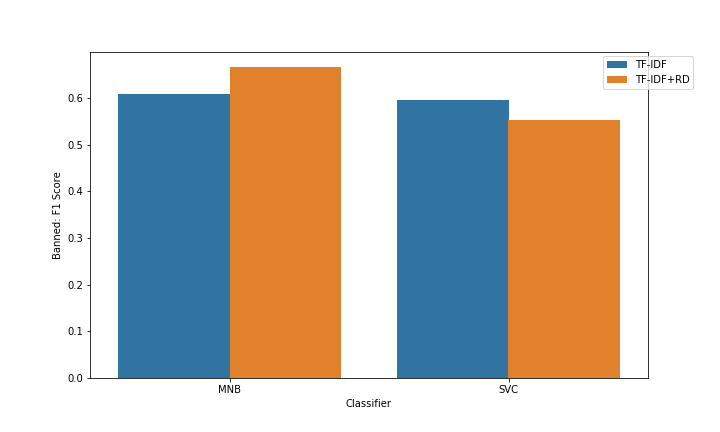
\includegraphics[width=0.6\textwidth]{posts_clf_barplot.png}
\end{figure}

\begin{figure}[H]
    \caption{Threads: SVM vs Naive Bayes, with and without Rank Divergence}
    \centering
    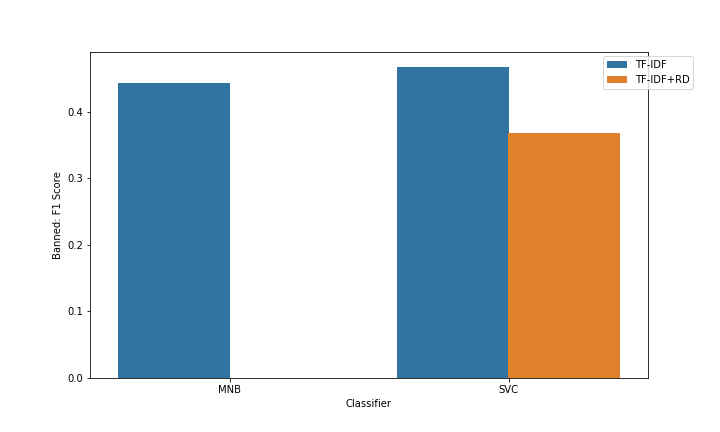
\includegraphics[width=0.6\textwidth]{threads_clf_barplot.png}
\end{figure}

\begin{figure}[H]
    \caption{Subreddits: SVM vs Naive Bayes, with and without Rank Divergence}
    \centering
    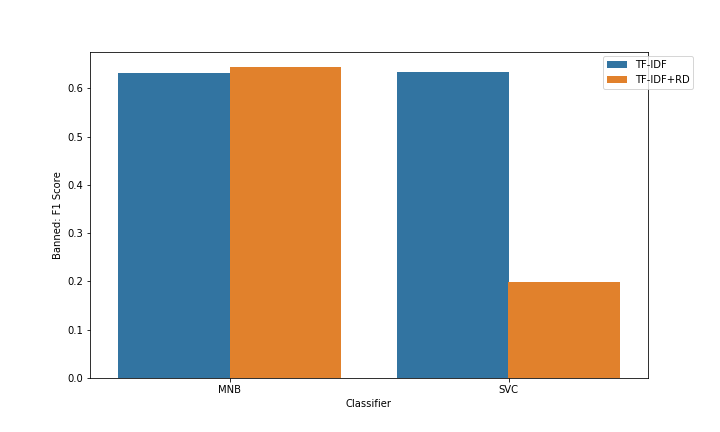
\includegraphics[width=0.6\textwidth]{subreddits_clf_barplot.png}
\end{figure}


\end{document}
